\section{Introduction}\label{sec:introduction}



\begin{figure*}[t]
\centering
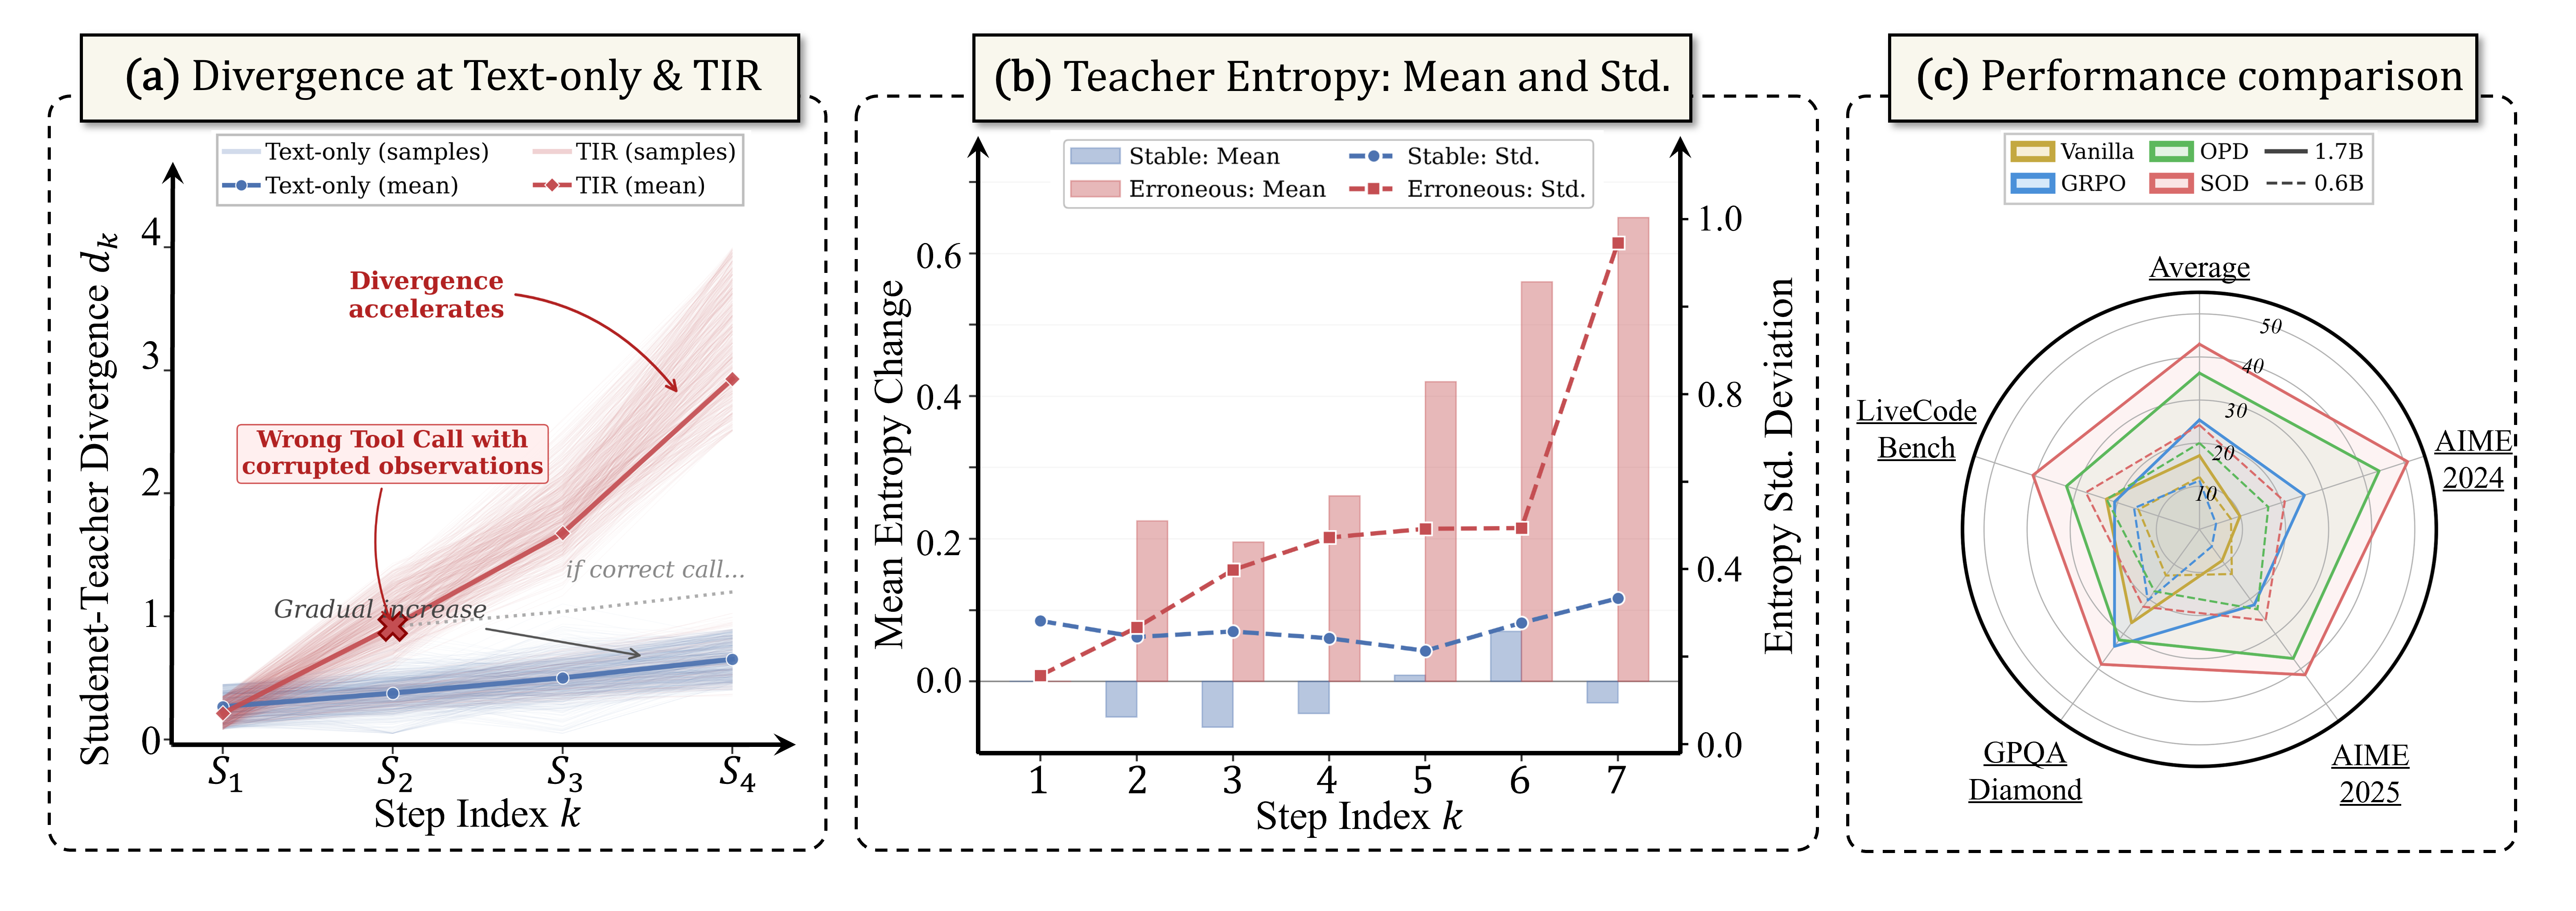
\includegraphics[width=1.0\linewidth]{pic/intro_v13.png}
\caption{\textbf{The motivation of \ourmodel}. 
(a) Student-teacher divergence $d_k$ across reasoning steps, sampled from 800 trajectories: in TIR, erroneous tool calls cause divergence to accelerate sharply, unlike the gradual drift in text-only reasoning. 
(b) Teacher entropy statistics over 800 sampled trajectories: on erroneous trajectories, both the mean entropy change (bars) and the standard deviation (dashed lines) grow rapidly at later steps, indicating increasingly unreliable teacher supervision. Please refer to~\Cref{app:H} for detailed cases.
(c) Radar chart comparing methods on four benchmarks.}
\label{motivation}
\vspace{-2 em}
\end{figure*}




Agentic capabilities have substantially expanded the applicability of large language models (LLMs)~\citep{xi2023rise,AgentDistillation}, enabling them to solve complex real-world tasks~\citep{react,schick2023toolformer,singh2025agentic}. 
However, such capabilities are typically realized by large-scale models, which incurs substantial inference cost, deployment overhead, and system complexity~\citep{singh2025agentic,chenglin2024mixed,fan2026agentprocessbench}. In latency-, resource-, and privacy-sensitive scenarios, transferring agentic capabilities to small language models (SLMs) that can be deployed on-device is therefore of significant practical importance~\citep{xu2024ondevice,xu2024kd_llm_survey,Agentdistill,oresearcher,coa}. Despite this motivation, enabling SLMs to acquire stable and effective tool-integrated reasoning (TIR) abilities remains a major challenge~\citep{qian2025toolrl,rainone2025replacing,xue2025simpletir,sad}.

Existing post-training methods for enhancing TIR abilities are largely based on reinforcement learning (RL)~\citep{li2025torl,jin2025searchr1,song2025r1searcher}, particularly policy optimization algorithms such as group relative policy optimization (GRPO)~\citep{grpo}. However, in SLM-based TIR settings, RL often suffers from unstable optimization~\citep{qian2025toolrl,rainone2025replacing}. TIR tasks typically involve long-horizon trajectories~\citep{li2025torl}, multi-step decision making~\citep{jin2025searchr1}, and interactions with external tools~\citep{singh2025agentic}, whereas RL commonly provides only sparse outcome-level rewards~\citep{deepseek2025r1}. For small models with limited capacity and weaker exploration ability, such sparse supervision can further exacerbate exploration failure, leaving the policy in a cold-start regime with few informative reasoning signals~\citep{kepo}.




Recently, on-policy distillation (OPD) has emerged as a promising paradigm for post-training~\citep{opd,gu2024minillm,eopd,ropd,lightOPD}. Unlike RL methods that rely on sparse, trajectory-level rewards~\citep{deepseek2025r1}, OPD provides dense token-level supervision~\citep{gu2024minillm} on trajectories sampled from the student's own policy~\citep{opd}, thereby alleviating the credit assignment difficulty inherent in sparse reward signals~\citep{qwen2025qwen3,li2026rethinking} while substantially improving sample efficiency~\citep{xu2026rlkd} and training stability~\citep{qwen2025qwen3}.














However, our experiments show that directly transferring OPD to SLM-based TIR can lead to severe training instability~\citep{srpo,sdrlvr,bousselham2025vold,wang2026openclaw}. We attribute this failure to a fundamental difference between how student trajectories deviate from the teacher distribution in TIR and in standard text-based reasoning~\citep{li2026rethinking,fu2026revisiting,opdsurvey,bousselham2025vold}. As illustrated in~\cref{motivation}(a), in text-only reasoning, even when the student gradually departs from the teacher, subsequent states still evolve continuously along the generated context, and the resulting distribution shift is typically progressive~\citep{ross2011reduction,opd}. In contrast, TIR introduces discontinuous state transitions through tool interactions~\citep{li2025torl}. A single erroneous tool call can inject an incorrect observation into the context, causing subsequent reasoning steps to unfold from a corrupted state~\citep{qian2025toolrl}. This issue is further amplified because teacher models are often highly accurate in tool use, whereas small models have limited capacity and weaker exploration ability~\citep{gudibande2024false,rainone2025replacing}. During early training, small models may accumulate multiple erroneous tool calls, causing their state distribution to rapidly drift away from the teacher distribution~\citep{li2026rethinking,wang2026tcod}. In such out-of-distribution states, teacher-provided token-level supervision may become unreliable or even misleading~\citep{veto,bousselham2025vold,kepo,tip,srpo} as illustrated in~\cref{motivation}(b), and the enlarged student-teacher discrepancy can induce unstable gradients and even training collapse~\citep{li2026rethinking,qwen2025qwen3}.


Based on this observation, we propose \textbf{\ourmodel}, a 
\textbf{S}tep-wise \textbf{O}n-policy \textbf{D}istillation framework for small language model agents. The core idea is to adaptively adjust the distillation strength at each reasoning step according to the divergence between the student and teacher. Specifically, when the student remains well aligned with the teacher, \ourmodel preserves dense supervision to fully exploit teacher guidance; when the deviation becomes large, it progressively attenuates the distillation signal for the corresponding step, thereby reducing the influence of potentially misleading supervision under out-of-distribution states. 
Experimental results (as displayed in~\cref{motivation}(c)) demonstrate that this simple yet effective step-wise reweighting mechanism enables lightweight agents to acquire agentic TIR capabilities more efficiently. 
Extensive experiments on challenging math, science, and code benchmarks show that \ourmodel outperforms the second-best baseline by up to \textbf{20.86\%}.
Notably, our 0.6B-scale student achieves \textbf{26.13\%} accuracy on AIME 2025. To our best knowledge, this is the first sub-billion-parameter model to reach this level on such a challenging reasoning benchmark.










